\chapter{Extra-Credit Question 4}
\label{available-representation}

\textbf{Repeat question 2, but change ``followers'' to ``following''?  In other words, are the people I am following following more people?}

\begin{itemize}
\item Using the `userFollowerData' file generated in question 2 as input, I extracted the following \textunderscore count from the JSON structure and stored it in a file `followingCount'. This code is listed in Listing \ref{lst:q4code1}
\item I calculated the mean, median and standard deviation for the following count. This code is listed in Listing \ref{lst:q4code2}. The output of mean, median and standard deviation are given in Table \ref{Table:q4table1}

\begin{table}

\caption{Mean, Median and Standard Deviation of number of people followed by the people followed by `ohttic'}
\label{Table:q4table1}
\begin{center}
\begin{tabular}{| c | c |}
\hline
Key & Value \\ \hline

Mean & 45183.2 \\ \hline
Median & 4609.5 \\ \hline
Standard Deviation & 96280.5156542 \\ \hline

\hline

\end{tabular}
\end{center}
\end{table}

\newpage
\item I created a graph with following count on y-axis and the friends themselves on x-axis including `ohttic'. The graph is summarized in Figure \ref{fig:q4fig2}.
\begin{figure}[h!]
\begin{center}
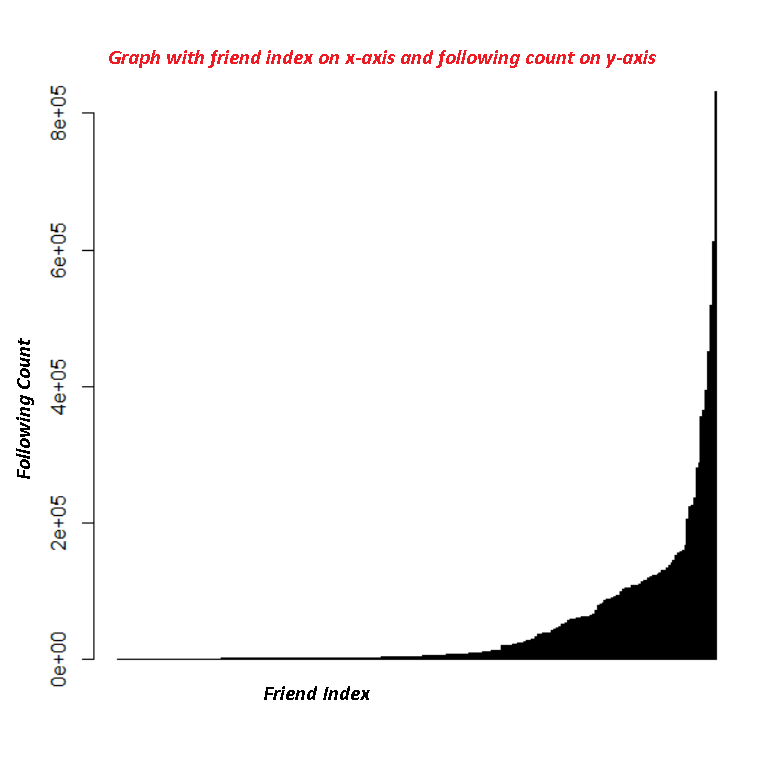
\includegraphics[scale=0.55, keepaspectratio=true]{figures/followingWithoutLog.PNG}
\caption{Graph with following count on y-axis and the friend index on x-axis }
\label{fig:q4fig2}
\end{center}
\end{figure}
\newpage
\item From the calculated median value `4609.5' and following count of `ohttic' `1,923' we can say that `ohttic' have less following count than his friends.
\ref{fig:q4fig2}.
\begin{figure}[h!]
\begin{center}
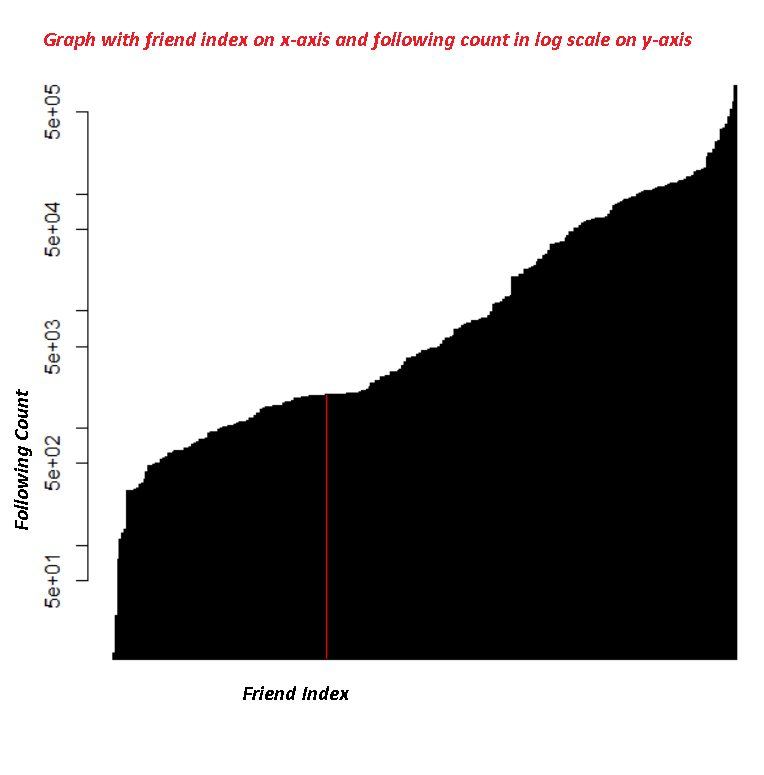
\includegraphics[scale=0.55, keepaspectratio=true]{figures/following.PNG}
\caption{Graph with following count in log scale on y-axis and the friend index on x-axis }
\label{fig:q4fig3}
\end{center}
\end{figure}
\end{itemize}

\newpage
\textbf{Code Listing}
\lstinputlisting[language=Python,caption=Python code for extracting friends count from JSON structure,frame=single,label=lst:q4code1,breaklines=true,captionpos=b,numbers=left,showspaces=false,showstringspaces=false,basicstyle=\footnotesize]{src/extractFollowing.py}

\textbf{Code Listing}
\lstinputlisting[language=Python,caption=Python code for calculating mean median and standard deviation,frame=single,label=lst:q4code2,breaklines=true,captionpos=b,numbers=left,showspaces=false,showstringspaces=false,basicstyle=\footnotesize]{src/getMeanMedianStandardDeviation3.py}
